
%(BEGIN_QUESTION)
% Copyright 2008, Tony R. Kuphaldt, released under the Creative Commons Attribution License (v 1.0)
% This means you may do almost anything with this work of mine, so long as you give me proper credit

The following strobe light has a problem: the flash tube never flashes.

$$\includegraphics[width=15.5cm]{i03188x01.eps}$$

Turning the flash rate control (rheostat $R_1$) to the slowest position, you take two voltage measurements with a voltmeter: at test point 3 (between TP3 and ground) you measure a voltage rhythmically pulsating between about 1.5 and 4 volts DC.  At test point 6 (between TP6 and ground) you measure a voltage rhythmically pulsating between about 0.3 and 6 volts DC.

From this information, identify two possible faults (either one of which could account for the problem and all measured values in this circuit), and also identify two circuit elements that could not possibly be to blame (i.e. two things that you know {\it must} be functioning properly, no matter what else may be faulted) other than the 6 volt battery and the on/off switch.  The circuit elements you identify as either possibly faulted or properly functioning can be wires, traces, and connections as well as components.  Be as specific as you can in your answers, identifying both the circuit element and the type of fault.

\medskip
\goodbreak
\item{} Circuit elements that are possibly faulted
\item{1.}
\item{2.} 
\end{itemize}

\medskip
\goodbreak
\item{} Circuit elements that must be functioning properly
\item{1.} 
\item{2.} 
\end{itemize}

\vfil 

\underbar{file i03188}
\eject
%(END_QUESTION)





%(BEGIN_ANSWER)

This is a graded question -- no answers or hints given!

%(END_ANSWER)





%(BEGIN_NOTES)

Note: the following answers are not exhaustive.  There may be more circuit elements possibly at fault and more circuit elements known to be functioning properly!

\begin{itemize}
\item{} Circuit elements that are possibly faulted
\item{1.} Secondary winding of transformer $T_1$ failed open
\item{2.} Failed flash tube (either open or shorted)
\end{itemize}

\begin{itemize}
\item{} Circuit elements that must be functioning properly (besides power supply and signal source)
\item{1.} Rheostat $R_1$
\item{2.} Resistor $R_2$
\item{3.} Capacitor $C_1$
\item{4.} All transistors
\end{itemize}

%INDEX% Troubleshooting review: electric circuits

%(END_NOTES)


